% VUT FIT MITAI
% MSZ 2021/2022
% Author: Vladimir Dusek
% Login: xdusek27

%%%%%%%%%%%%%%%%%%%%%%%%%%%%%%%%%%%%%%%%%%%%%%%%%%%%%%%%%%%%%%%%%%%%%%%%%%%%%%%%

% Path to figures
\graphicspath{{msp/odhady_parametru/figures}}

%%%%%%%%%%%%%%%%%%%%%%%%%%%%%%%%%%%%%%%%%%%%%%%%%%%%%%%%%%%%%%%%%%%%%%%%%%%%%%%%

\chapter{MSP~--~Bodové a intervalové odhady parametrů, testování hypotéz o parametrech.}

%%%%%%%%%%%%%%%%%%%%%%%%%%%%%%%%%%%%%%%%%%%%%%%%%%%%%%%%%%%%%%%%%%%%%%%%%%%%%%%%

\section{Zdroje}

\begin{compactitem}
    \item \path{MSP_pred_02_Opakovani_Statistika_Regrese.}pdf
    \item \path{MSP_pred_03_Norm-Bi_Odhady-Testy.pdf}
    \item Wikipedia
\end{compactitem}

%%%%%%%%%%%%%%%%%%%%%%%%%%%%%%%%%%%%%%%%%%%%%%%%%%%%%%%%%%%%%%%%%%%%%%%%%%%%%%%%

\section{Úvod a kontext}

\begin{compactitem}
    \item \textbf{Náhodný výběr} -- Z celého stavového prostoru jsou náhodně vybrány vzorky (je proveden náhodný výběr). \begin{compactitem}
        Např. princip volebních průzkumů.
    \end{compactitem}

    \item Na statistický soubor $(x_1, x_2, \ldots, x_n)$ můžeme nahlížet jako na výběrový soubor získaný náhodným výběrem z náhodné proměnné $X$. \begin{compactitem}
        \item Stejným způsobem pro vícerozměrné statistické soubory. Soubor\break $((x_1, y_1), (x_2, y_2), \ldots, (x_n, y_n))$ může být získán náhodným výběrem ze dvou náhodných proměnných $X, Y$.
    \end{compactitem}

    \item Cílem je, na základě statistického souboru $(x_1, x_2, \ldots, x_n)$ odhadnout parametry náhodné proměnné $X$. \begin{compactitem}
        \item Typicky jde o číselné charakteristiky jako jsou střední hodnota a rozptyl.
    \end{compactitem}

    \item Jako \textbf{statistickou hypotézu} chápeme určitý předpoklad o rozdělení náhodných veličin. Jestliže se tyto předpoklady týkají hodnot parametrů rozdělení náhodné veličiny, pak hovoříme o parametrických hypotézách. V opačném případě se jedná o hypotézy neparametrické.

    \item \textbf{Parametrické testy} -- Předpokládají nějaké rozdělení pravděpodobnosti, hypotéza je o parametrech rozdělení základního souboru. \begin{compactitem}

        \item Hypotézy o parametru jednoho základního souboru -- střední hodnota, mediána, rozptyl, \dots
        \item Hypotézy o parametrech dvou základních souborů
        (srovnávací testy) -- rovnost středních hodnot, rovnost
        rozptylů, \dots
    \end{compactitem}

    \item \textbf{Neparametrické testy} -- Nepředpokládají žádné rozdělení pravděpodobnosti, hypotéza je o jiných vlastnostech základního souboru. \begin{compactitem}
        \item Hypotéza o tvaru rozdělení, závislosti proměnných, \dots
    \end{compactitem}

\end{compactitem}

%%%%%%%%%%%%%%%%%%%%%%%%%%%%%%%%%%%%%%%%%%%%%%%%%%%%%%%%%%%%%%%%%%%%%%%%%%%%%%%%

\section{Bodový odhad}

\begin{compactitem}
    \item Bodový odhad aproximuje hledaný parametr jednou číselnou hodnotou (jde o nejlepší odhad). \begin{compactitem}
        \item To se hodí zejména pokud je parametr potřeba pro další výpočty.
    \end{compactitem}

    \item Formálně; nechť $(X_1, X_2, \ldots, X_n)$ je náhodný výběr z rozdělení s distribuční funkcí $F( x, \theta)$. Statistika $T(X_1, X_2, \ldots, X_n)$ se nazývá bodovým odhadem parametru $\theta$, pokud nabývá hodnot blízkých parametru $\theta$.

    \item Vlasnoti: \begin{compactitem}
        \item Bodový odhad T se nazývá nestranný (nevychýlený), pokud platí:
        $$ E(T) = \theta $$
        \item Bodový odhad T se nazývá stranný (vychýlený), pokud platí:
        $$ E(T) \not= \theta $$
        \item Bodový odhad T se nazývá konzistentní, pokud platí:
        $$ \lim_{n \rightarrow \infty}{P(|T(X_1, X_2, \ldots, X_n) - \theta|} < \epsilon) = 1 $$
    \end{compactitem}

    \item Máme metody pro bodové odhady parametrů pro jednotlivá pravděpodobnostní rozdělení (Normální, Binomické, \dots).
\end{compactitem}

%%%%%%%%%%%%%%%%%%%%%%%%%%%%%%%%%%%%%%%%%%%%%%%%%%%%%%%%%%%%%%%%%%%%%%%%%%%%%%%%

\section{Intervalový odhad}

\begin{compactitem}
    \item Intervalový odhad aproximuje hledaný parametr intervalem. Tj. hledaný parametr se s předem stanovenou spolehlivostí nachází uvnitř výsledného intervalu. \begin{compactitem}
        \item To se hodí, pokud potřebujeme znát přesnost odhadu parametru.
        \item Bodový odhad je intervalový odhad se spolehlivostí 0.
    \end{compactitem}

    \item Formálně; nechť $X$ je náhodná proměnná, která má distribuční funkci $F( x, \theta)$. Interval spolehlivosti pro parametr $\theta$ na hranici spolehlivosti $1 - \alpha ~,~ \alpha \in \langle 0, 1 \rangle$ je dvojice statistik $T_1$, $T_2$, pro které platí:
    $$ P(T_1 \leq \theta \leq T_2) = 1 - \alpha $$
    Intervalový odhad parametru $\theta$ se spolehlivostí $1 - \alpha ~,~ \alpha \in \langle 0, 1 \rangle$ je interval $\langle t_1, t_2 \rangle$, kde $t_1$, resp. $t_2$ je realizací statistiky $T_1$, resp. $T_2$.

    \item Požadavky na intervalový odhad: \begin{compactitem}
        \item aby pravděpodobnost $1 - \alpha$ byla co největší;
        \item interval byl co nejmenší.
        \item Typicky volíme $\alpha \in \{ 0,1, 0,05, 0,01 \}$.
    \end{compactitem}

    \item Máme metody pro intervalové odhady parametrů pro jednotlivá pravděpodobnostní rozdělení (Normální, Binomické, \dots).
\end{compactitem}

%%%%%%%%%%%%%%%%%%%%%%%%%%%%%%%%%%%%%%%%%%%%%%%%%%%%%%%%%%%%%%%%%%%%%%%%%%%%%%%%

\section{Testování hypotéz o parametrech}

\begin{compactitem}
    \item Testování statistických hypotéz umožňuje posoudit, zda experimentálně získaná data vyhovují předpokladu, který jsme před provedením testování učinili. Můžeme například posuzovat, zda platí předpoklad, že určitý lék je účinnější než jiný; nebo zda platí, že úroveň matematických dovedností žáků 9. tříd je nezávislá na pohlaví a na regionu.

    \item \textbf{Statistická hypotéza} $H$ je tvrzení o vlastnostech pravděpodobnostního rozdělení zkoumané náhodné proměnné $X$ s distribuční funkcí $F(x, \theta)$. \begin{compactitem}
        \item Postup kterým hypotézu ověřujeme, se nazývá test statistické hypotézy.
    \end{compactitem}

    \item Jako alternativu vůči hypotéze postavíme tzv. \textbf{alternativní hypotézu} $H_A$ (také nulová hypotéza), kterou volíme v kontextu dané úlohy. \begin{compactitem}
        \item $H_0 : \theta = \theta_0$ je hypotéza, že parametr $\theta$ má hodnotu $\theta_0$
        \item $H_A : \theta > \theta_0$ je jednostranná alternativní hypotéza.
        \item $H_A : \theta \not= \theta_0$ je oboustranná alternativní hypotéza.
    \end{compactitem}

    \item Pro testování hypotézy $H$ proti nějaké zvolené alternativní hypotéze $H_A$ se konstruuje vhodná statistika $T(X_1, X_2, \ldots, X_n)$, tzv. \textbf{testové kritérium}.

    \item Při hledání testového kritéria $T$ se vychází z požadavků na zamítnutí hypotézy $H$. Zajímá nás, za jakých podmínek lze hypotézu zamítnout. K tomu se konstruuje množina možných hodnot realizace statistiky $T$. Tato množina se nazývá kritický obor a označuje se $W_{\alpha}$. Velikost této množiny závisí na spolehlivosti našeho tvrzení (parametr $\alpha$ -- hladina významnosti). \begin{compactitem}
        \item Pokud realizace zvolené statistiky $t = T(x_1, x_2, \ldots, x_n)$ padne do kritického oboru $W_{\alpha}(t \in W_{\alpha})$ říkáme, že \textbf{hypotézu zamítáme} na hladině významnosti $\alpha$.
    \end{compactitem}

    \item U většiny testů se místo kritického oboru udává doplněk kritického oboru $\overline{W}_{\alpha}$. \begin{compactitem}
        \item $\overline{W}_{\alpha} = \mathbb{R} \setminus W_{\alpha}$.
        \item Pokud realizace zvolené statistiky $T$ padne do doplňku kritického oboru $t \in \overline{W}_{\alpha}$ říkáme, že \textbf{hypotézu nezamítáme} na hladině významnosti $\alpha$.
    \end{compactitem}

    \item Nezamítnutí hypotézy $H$, resp. $H_A$, neznamená ještě prokázání její platnosti, neboť jsme na základě realizace náhodného výběru získali pouze informace, které nestačí na její zamítnutí. Je-li to možné, je vhodné před přijetím dané hypotézy zvětšit rozsah statistického souboru a znovu hypotézu $H$ testovat.

    \begin{figure}[H]
        \centering
        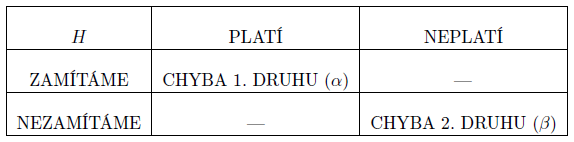
\includegraphics[width=0.75\linewidth]{hypoteza.png}
        \caption{Testování hypotézy.}
    \end{figure}

    \item Chybu 1. druhu ($\alpha$) si volíme, chyba 2. druhu závisí na typu testu a na parametrech. Hodnota $1 - \beta$ se nazývá síla testu.

    \item Pro konkrétní rozdělení budeme u testů uvádět realizaci testovacího kritéria $t = T( x_1, x_2, \ldots, x_n)$ a doplněk kritického oboru $\overline{W}_{\alpha}$ vzhledem k příslušné alternativní hypotéze.

    \item Existují různé druhy testů pro různé typy hypotéz v závislosti na rozdělení.
\end{compactitem}

%%%%%%%%%%%%%%%%%%%%%%%%%%%%%%%%%%%%%%%%%%%%%%%%%%%%%%%%%%%%%%%%%%%%%%%%%%%%%%%%

\section{Základní testy hypotéz pro vybraná rozdělení}

\subsection{Jeden výběr z Normálního rozdělení}

\begin{compactitem}
    \item Máme realizi náhodného výběru $(x_1, x_2, \ldots, x_n)$ pro náhodnou proměnnou $X$ a předpokládáme, že $X \sim N(\mu, \sigma^2)$.

    \item Testujeme zda daná realizace náhodného výběru odpovídá danému normálnímu rozdělení.

    \item Testujeme: \begin{compactitem}
        \item střední hodnotu, např. Studentův jednovýběrový test;
        $$ H_0 : \mu = \mu_0 $$
        \item rozptyl, např. Test na rozptyl.
        $$ H_0 : \sigma^2 = \sigma_0^2 $$
    \end{compactitem}

    \item Pro výběr z 2-rozměrného Normálního rozdělení jsou jiné testy (např. Studentův párový test).
\end{compactitem}

\subsection{Dva výběry z Normálního rozdělení}

\begin{compactitem}
    \item Máme realizi náhodného výběru $(x_1, x_2, \ldots, x_n)$ pro náhodnou proměnnou $X$ a $(y_1, y_2, \ldots, y_m)$ pro náhodnou proměnnou $Y$. Předpokládáme, že $X \sim N(\mu_X, \sigma_X^2)$ a $Y \sim N(\mu_Y, \sigma_Y^2)$.

    \item Testujeme zda realizace náhodného výběru $(x_1, x_2, \ldots, x_n)$ a $(y_1, y_2, \ldots, y_n)$ odpovídá stejnému normálnímu rozdělení.

    \item Testujeme: \begin{compactitem}
        \item rovnost rozptylů, např. F-test;
        $$ H_0 : \sigma_X^2 = \sigma_Y^2 $$

        \item střední hodnotu, např. Studentův dvouvýběrový test za podmínky $\sigma_X^2 = \sigma_Y^2$;
        $$ H_0 : \mu_X - \mu_Y = \mu_0 $$

    \end{compactitem}
\end{compactitem}

\subsection{Jeden výběr z Binomického rozdělení}

\begin{compactitem}
    \item Předpokládáme, že $X \sim Bi(1, p)$, neznámý parametr je $p$, provedeme $n$  měření / pokusů a získáme realizi náhodného výběru $(x_1, x_2, \ldots, x_n)$ pro náhodnou proměnnou $X$.

    \item Testujeme zda realizace náhodného výběru $(x_1, x_2, \ldots, x_n)$ odpovídá danému binomickému rozdělení.

    \item Testujeme: \begin{compactitem}
        \item pravděpodobnost $p$
        $$ H_0 : p = p_0 $$
    \end{compactitem}
\end{compactitem}

\subsection{Dva výběry z Binomického rozdělení}

\begin{compactitem}
    \item Předpokládáme, že $X \sim Bi(1, p_X)$ a $Y \sim Bi(1, p_Y)$. Z každého provedeme několik měření / pokusů. Získáme realizaci náhodných výběrů $X: (x_1, x_2, \ldots, x_n)$ a $Y: (y_1, y_2, \ldots, y_m)$.

    \item Testujeme zda realizace náhodného výběru $X : (x_1, x_2, \ldots, x_n)$ a $Y: (y_1, y_2, \ldots, y_m)$ odpovídá stejnému binomickému rozdělení.

    \item Testujeme: \begin{compactitem}
        \item shodnost pravděpodobností $p_X$ a $p_Y$:
        $$ H_0 : p_X = p_Y $$
    \end{compactitem}
\end{compactitem}
